\usepackage{etex} %эта магическая херь избавляет от переполнения регистров TeX а!!!

\mode<article>{\usepackage{fullpage}}
\mode<presentation>{
    \usetheme{Madrid}
    \useoutertheme{shadow}
} 

\usepackage[utf8]{inputenc}
\usepackage[russian]{babel}
\usepackage{indentfirst}
\usepackage{graphicx}

\usepackage{amsmath}
\usepackage{amsfonts}
\usepackage{amsthm}
%\usepackage{algorithm}
%\usepackage{algorithmic}

%\usepackage[all]{xy}

\date{Лекция по дисциплине <<методы и средства защиты компьютерной информации>> (\today)}
\author[М.~М.~Шихов]{Михаил Шихов \\ \texttt{\underline{m.m.shihov@gmail.com}}}

%%для рисования графов пакетом xy-pic
%\entrymodifiers={++[o][F-]}

%%для псевдокода алгоритмов (algorithm,algorithmic)
%\renewcommand{\algorithmicrequire}{\textbf{Вход:}}
%\renewcommand{\algorithmicensure}{\textbf{Выход:}}
%\renewcommand{\algorithmiccomment}[1]{// #1}
%\floatname{algorithm}{Псевдокод}

%\setbeamercolor{alerted text}{fg=-green} %gyan, blue, green, -green

\title[Методы аппаратной защиты]{Методы защиты на аппаратном уровне}


\begin{document}


%титул и содержание статьи
\mode<article>{\maketitle\tableofcontents}

%титул и содержание презентации
\frame<presentation>{\titlepage}
\begin{frame}<presentation>[allowframebreaks]
\frametitle{Содержание}
\tableofcontents
\end{frame}


\section{Имя первой секции}

%аппаратная защита. 
%защищенный режим проца. защита памяти, привилегированный режим.
%организация программных сущностей (обработка исключений)
%i-button --- защита памяти


\begin{frame}
\frametitle{Контроль доступа}
\begin{definition}%theorem, lemma, proof, corollary, example
\alert{Контроль доступа} подразумевает активную система контроля, через которую проходят все запросы на доступ субъектов к объектам.
\end{definition}
Различают следующие модели систем контноля доступа.
\begin{itemize}
    \item Discretionary access control (DAC). Дискреционные или избирательные.
    \item Mandatory access control (MAC). Мандатные или полномочные.
    \item Role-based access control (RBAC). Ролевые. 
\end{itemize}
\end{frame}


Снова текст статьи первой секции.


\subsection[Кратко о подсекции]{Подсекция}


%вставка графики
\begin{frame}
\frametitle{Монитор доступа}
\begin{figure}
    \begin{center}
        \mode<presentation>{ 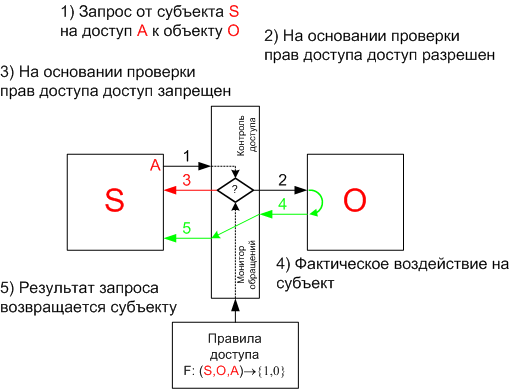
\includegraphics[height=.8\textheight]{pict/AccessControl} }
        \mode<article>{ 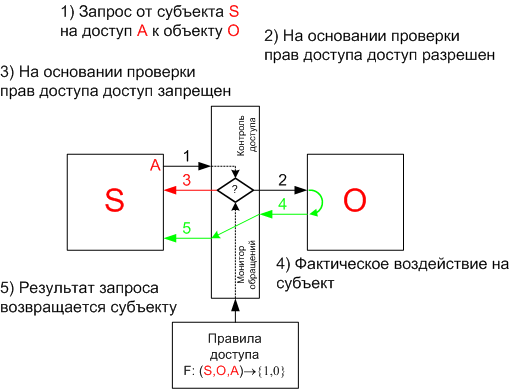
\includegraphics[width=.8\textwidth]{pict/AccessControl} } 
    \end{center}
\end{figure} 
\end{frame}


%оверлей
\begin{frame}
\frametitle{There Is No Largest Prime Number}
\framesubtitle{The proof uses \textit{reductio ad absurdum}.}
\begin{theorem}
    There is no largest prime number.
\end{theorem}
\begin{proof}
    \begin{enumerate}
        \item<1-> Suppose $p$ were the largest prime number.
        \item<2-> Let $q$ be the product of the first $p$ numbers.
        \item<3-> Then $q + 1$ is not divisible by any of them.
        \item<1-> Thus $q + 1$ is also prime and greater than $p$.\qedhere
    \end{enumerate}
\end{proof}
\uncover<4->{The proof used \textit{reductio ad absurdum}.}
\end{frame}


%в две колонки
\begin{frame}
    \frametitle{What’s Still To Do?}
    
    \begin{columns}
        \column{.5\textwidth}
            \begin{block}{Answered Questions}
                How many primes are there?
            \end{block}
        
        \column{.5\textwidth}
            \begin{block}{Open Questions}
                Is every even number the sum of two primes? \cite{bib:fsb}
            \end{block}
    \end{columns}
\end{frame}


%сводка по ссылкам
\begin{frame}
    \frametitle{Источники}
    \begin{itemize}
        \item ФСБ: \cite{bib:fsb}
        \item ФСТЭК: \cite{bib:fstec}
    \end{itemize}
\end{frame}


%слайд раскладывается на несколько: allowframebreaks
\begin{frame}[allowframebreaks]{Библиография}
\begin{thebibliography}{99}
    \bibitem{bib:fsb}www.fsb.ru
    \bibitem{bib:fstec}www.fstec.ru
\end{thebibliography}
\end{frame}


\appendix
Что нужно знать, но в этой презентации этого нет. Секции, слайды


\end{document}